\documentclass[
    % aspectratio=169,                   % 使用 16:9 比例
]{beamer}
\mode<presentation>
\usetheme[
    % navigation=subsections,            % 使用子章节进度导航
    % lang=en,                           % 使用英文logo
    % cjk=true,                          % 使用CJK而不是ctex
    % color=red,                         % 使用红色主题
    % pattern=none,                      % 不使用图案装饰
]{SJTUBeamer}

\title{\textsf{SJTUBeamer} 幻灯片模板}  % 标题
\subtitle{SJTUBeamer Template}         % 副标题
\author{Log Creative}                  % 作者
\institute[]{github.com/LogCreative}   % 组织
\date{\today}                          % 日期

\begin{document}

    \maketitle                         % 创建标题页

    \begin{frame}
        \frametitle{提纲}
        \tableofcontents               % 创建目录
    \end{frame}

\section{第 1 节}
\subsection{第 1 小节}
    \begin{frame}
        \frametitle{标题}

        \begin{itemize}
            \item 第 1 项
            \item 第 2 项\footnote{这是一个脚注。}
            \item 第 3 项
        \end{itemize}

    \end{frame}

    \begin{frame}
        \frametitle{标题}
        \framesubtitle{子标题}

        \begin{equation}
            x^2+2x+1=(x+1)^2
        \end{equation}
        
    \end{frame}

\section{第 2 节}
    \begin{frame}
        \frametitle{一些盒子}
        
        \begin{block}{盒子}
            这是一个盒子
        \end{block}

        \begin{alertblock}{注意}
            注意内容
        \end{alertblock}

        \begin{exampleblock}{示例}
            示例内容
        \end{exampleblock}
    \end{frame}

    \begin{frame}[fragile]          % 注意添加 fragile 标记
        \frametitle{代码块}
        % 代码块参数:语言,标题
        % 请减少代码初始的缩进
        \begin{codeblock}{c++}{C++代码}
#include<iostream>

int main(){
    // Console Output
    std::cout << "Hello, SJTU!" << std::endl;
    return 0;
}
        \end{codeblock}
    \end{frame}

    \begin{frame}
        \frametitle{图}
        \begin{figure}
            \centering
            \begin{stampbox}
                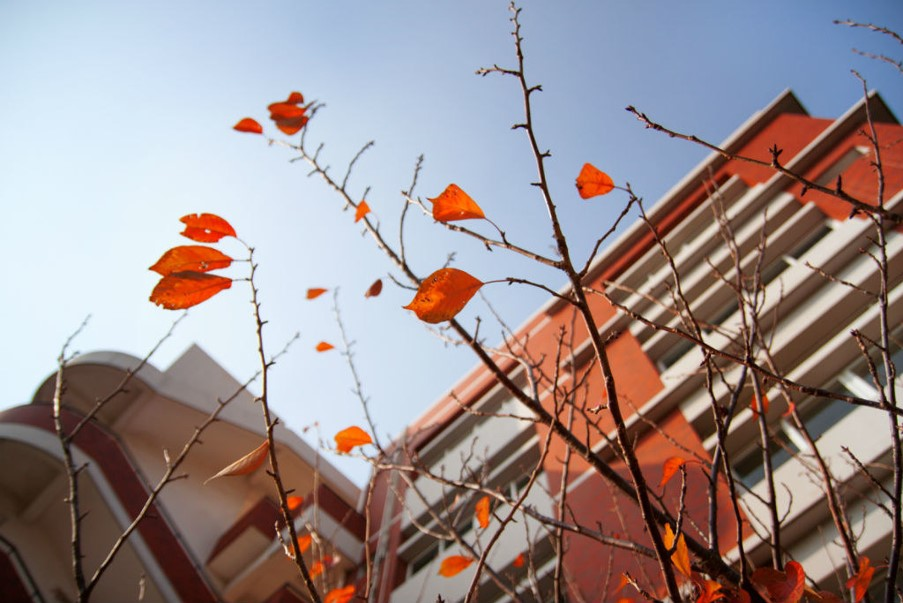
\includegraphics[height=0.3\textheight]{vi/plant.jpg}
            \end{stampbox}
            \caption{图片标题}
        \end{figure}
    \end{frame}

    \begin{frame}
        \frametitle{表与统计图}

        \begin{multicols}{2}
        \begin{table}
            \caption{表格标题}
            \pgfplotstabletypeset[
                columns/Quick/.style={dec sep align},
                columns/Cocktail/.style={dec sep align},
                column type=r,
                % fixed zerofill,
            ]{dat/test.csv}
        \end{table}
        
        \begin{figure}
            % !TeX root = ../test.tex
% Made with PGFPlotsEdt:
% https://logcreative.github.io/PGFPlotsEdt/
\begin{tikzpicture}
    \begin{axis}[
    width=\columnwidth,
    xlabel={$n$},
    ylabel={Average Steps},
    ymin={0},
    xmax={9},
    xmin={1},
    legend style={at={(0.5,1.03)},anchor=south},
    legend columns=2,
    grid,
    minor tick num=1]
     \pgfplotstableread {dat/test.csv}{\foo};           % read table
     \addplot+ [only marks] table[y=Quick] {\foo};
     \addplot+ [only marks] table[y=Cocktail] {\foo};
     \pgfplotsset{cycle list shift=-2};                 % start the cycle list from beginning
     \addplot+ [no markers,domain=1:9,] {1.502*x*ln(x)};
     \addplot+ [no markers,domain=1:9,] {0.4453*x*x-0.1365*x-0.473};
     \legend{Quick,CockTail,}                           % only mark the first two series
    \end{axis}
\end{tikzpicture}
            \caption{统计图标题}
        \end{figure}
        \end{multicols}
    \end{frame}

    \makebottom     % 创建尾页  % 非标准命令

\end{document}